%=========================================================================
% (c) 2014, 2015 Josef Lusticky

\section{Benchmarking methodology}\label{sec:analysis-metodology}
Procedures described by RFC~2544 can be used to measure the routing performance of the Linux kernel.
RFC~2544 specifies the benchmarking methodology for network interconnect devices.
The RFC~2544 specifies the following frame sizes to be used on Ethernet:
64, 128, 256, 512, 1024, 1280 and 1518~\cite{rfc2544}.
However, at least 66~B frame size must be used in case of UDP over IPv6 - the size of L2 header is 14,
the size of CRC is 4, the size of IPv6 header is 40 and the size of UDP header is 8.

In addition to the specified frame sizes, the Spirent TestCenter Application allows to configure custom iMix,
which can be used to define custom frame size distribution.
The Amsterdam Internet Exchange (AMS-IX) provides
statistics of the frame size distribution in the Internet traffic~\cite{amsix-frame-size}.
Figure~\ref{fig:analysis-amsix-frame-size} shows yearly frame size distribution provided by AMS-IX.
This distribution can be configured in the Spirent TestCenter Application, however,
to use the same iMix on both IPv4 and IPv6, the minimum frame size must be increased to 66 as described above.
\begin{figure}
	\centering
	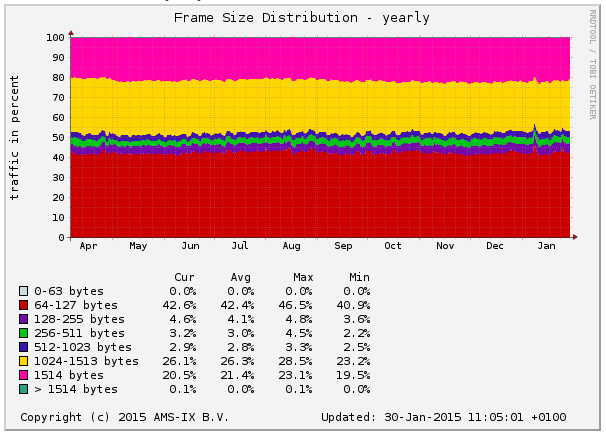
\includegraphics[width=14.5cm,keepaspectratio]{fig/amsix.png}
	\caption{Yearly frame size distribution at AMS-IX (source:~\cite{amsix-frame-size})}
	\label{fig:analysis-amsix-frame-size}
\end{figure}

The ideal way to implement the series of tests described in RFC~2544 is to use a tester
with both transmitting and receiving ports.
Connections are made from the sending ports of the tester to the receiving ports of the
device under test (DUT) and from the sending ports of the DUT back to the tester.
Figure~\ref{fig:analysis-rfc2544} shows the test implementation.   
Since the tester both sends the test traffic and receives
it back, after the traffic has been forwarded by the DUT, the tester
can easily determine if all of the transmitted packets were received
and verify that the correct packets were received~\cite{rfc2544}.
\begin{figure}
	\centering
	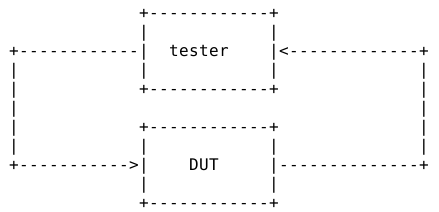
\includegraphics[width=9cm,keepaspectratio]{fig/rfc2544.png}
	\caption{RFC2544 test implementation (source:~\cite{rfc2544})}
	\label{fig:analysis-rfc2544}
\end{figure}

The Spirent TestCenter Application is able to display counters of transmitted and received frames on each interface.
The counters can be used to determine whether all of the transmitted packets on one interface were received
on the other interface and hence successfully forwarded by the server.
Unfortunately, the provided Spirent TestCenter Application contains no licence to perform the RFC 2544 throughput test
automatically, so the measurements must be configured manually in the Spirent TestCenter application.
The manual configuration consists of defining the transmit rate, observing the packet counters and comparing their values.
If the server forwards packets without a single loss, the transmit rate can be increased and the test repeated.
%Otherwise, the transmit rate must be decreased.
